Voici un problème classique des manuels scolaires de mathématiques pour collégiens ou lycéens français qui malgré sa grande simplicité va nous donner l'occasion de parler d'un petit biais classique en modélisation. Imaginons la situation suivante où M. CITER
\footnote{
	\emph{\og citer \fg} est l'anagramme de \emph{\og recti \fg} pour \emph{\og rectiligne \fg} comme les représentations sur le schéma.
}
doit amener, à l'aide d'un sceau, de l'eau de la rivière à l'abreuvoir d'un enclos pour ses vaches.

\smallskip
\begin{center}
	\fbox{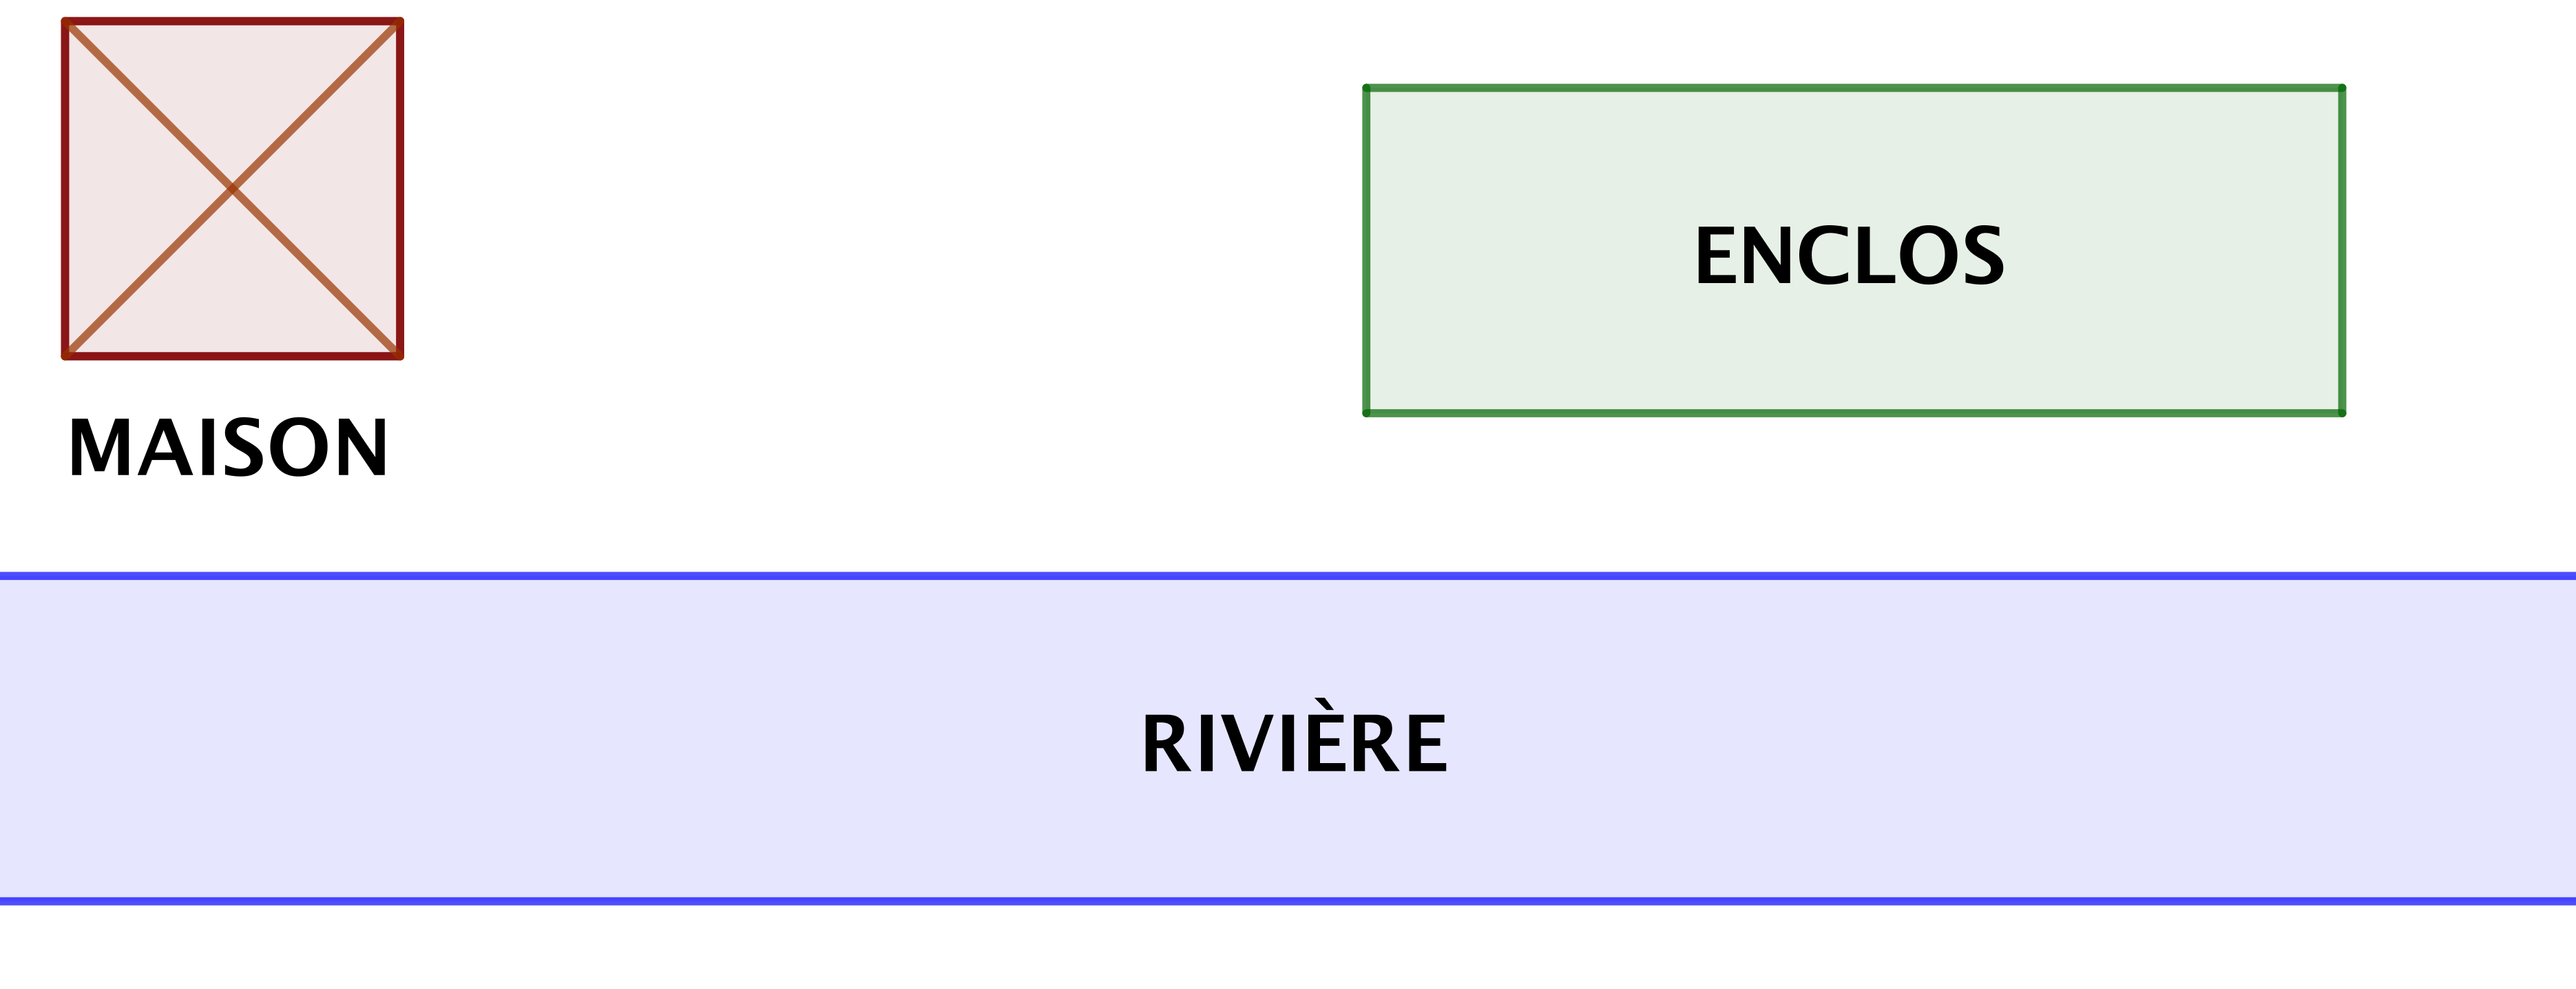
\includegraphics[scale = .6]{river-pb.png}}
\end{center}


\medskip


Commençons par simplifier un tout petit peu les données en ne gardant que la rive à laquelle M. CITER peut accéder, cette dernière étant symbolisée par la droite $\setproba{R}$ , ainsi qu'en réduisant la porte de la maison et l'abreuvoir des vaches aux points $P_M$ et $A_V$ respectivement. 

\smallskip
\begin{center}
	\fbox{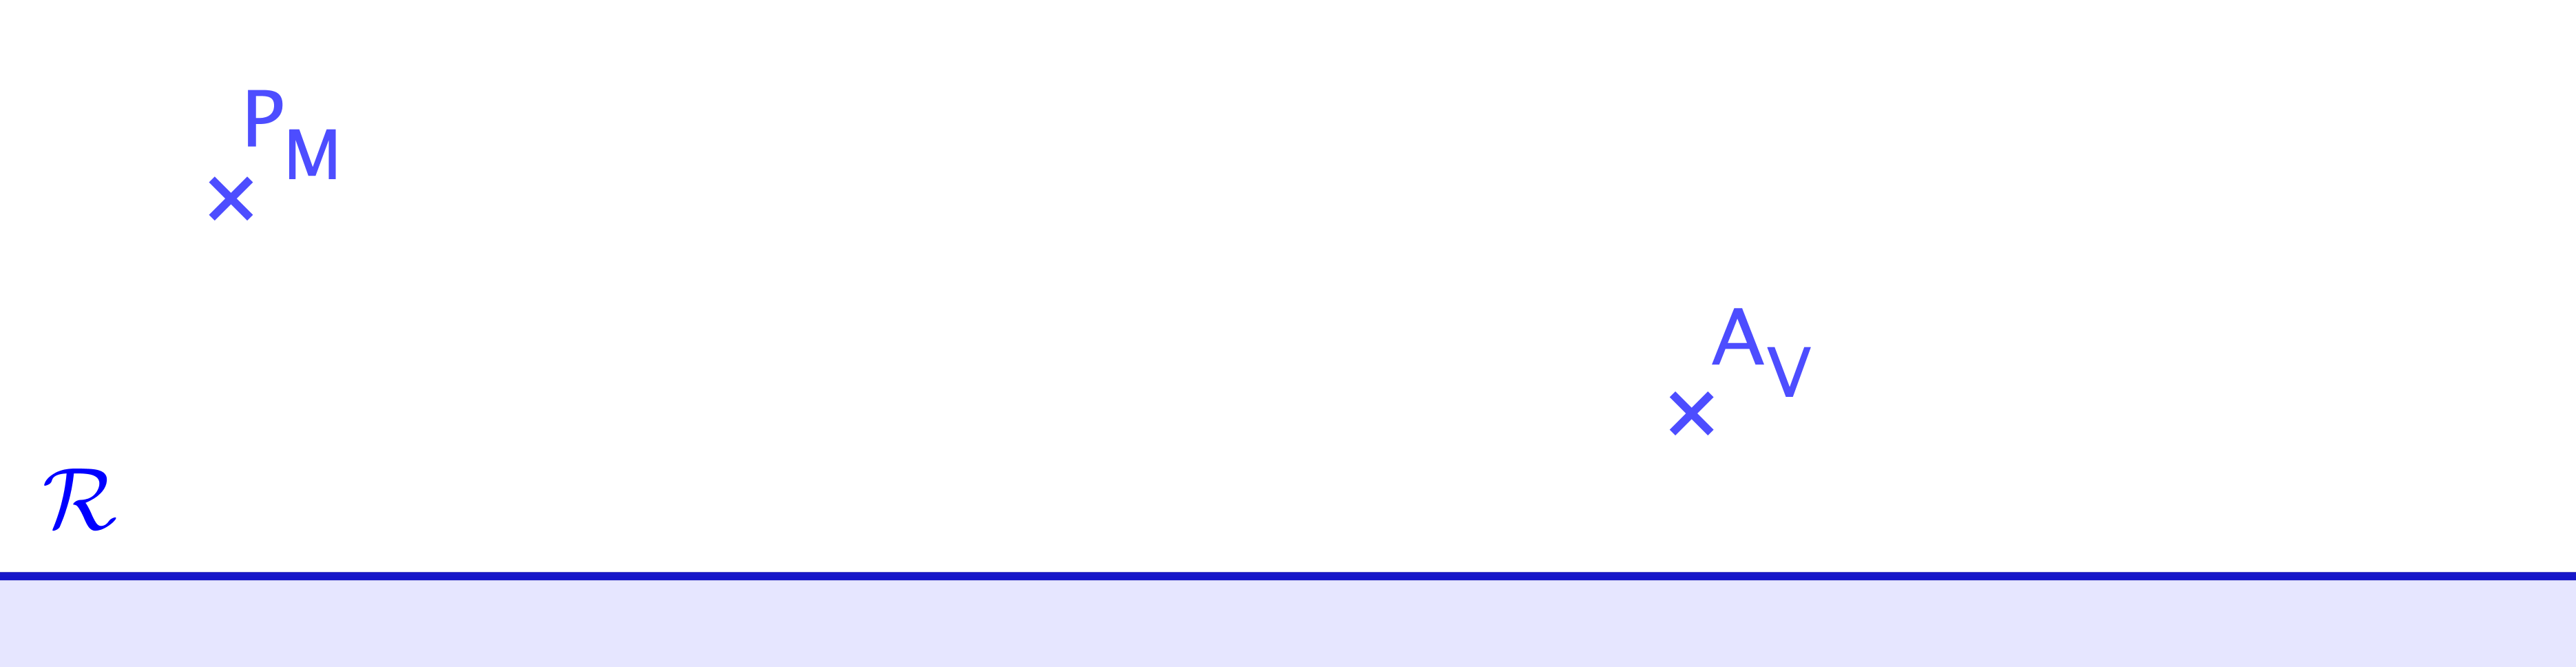
\includegraphics[scale = .6]{river-pb-simplified.png}}
\end{center}


\medskip


Une première solution consiste à chercher le chemin le plus court pour accéder à $A_V$ depuis $P_M$ en passant par la rive $\setproba{R}$ .
Ce problème a une solution géométrique très simple que voici
\footnote{
	Il existe une réponse analytique via l'étude des extrema de \emph{\og la fonction \fg} $E P_V + E A_V$ , un choix de fonction qui sous-entend que l'on ne passe qu'une fois à la rive, un point qu'il resterait à justifier proprement.
	De plus, techniquement il faut utiliser un théorème délicat d'existence de minimum car le signe de la dérivée n'est pas évident à déterminer. 
},
le point $E$ étant l'endroit où récupérer l'eau.

\smallskip
\begin{center}
	\fbox{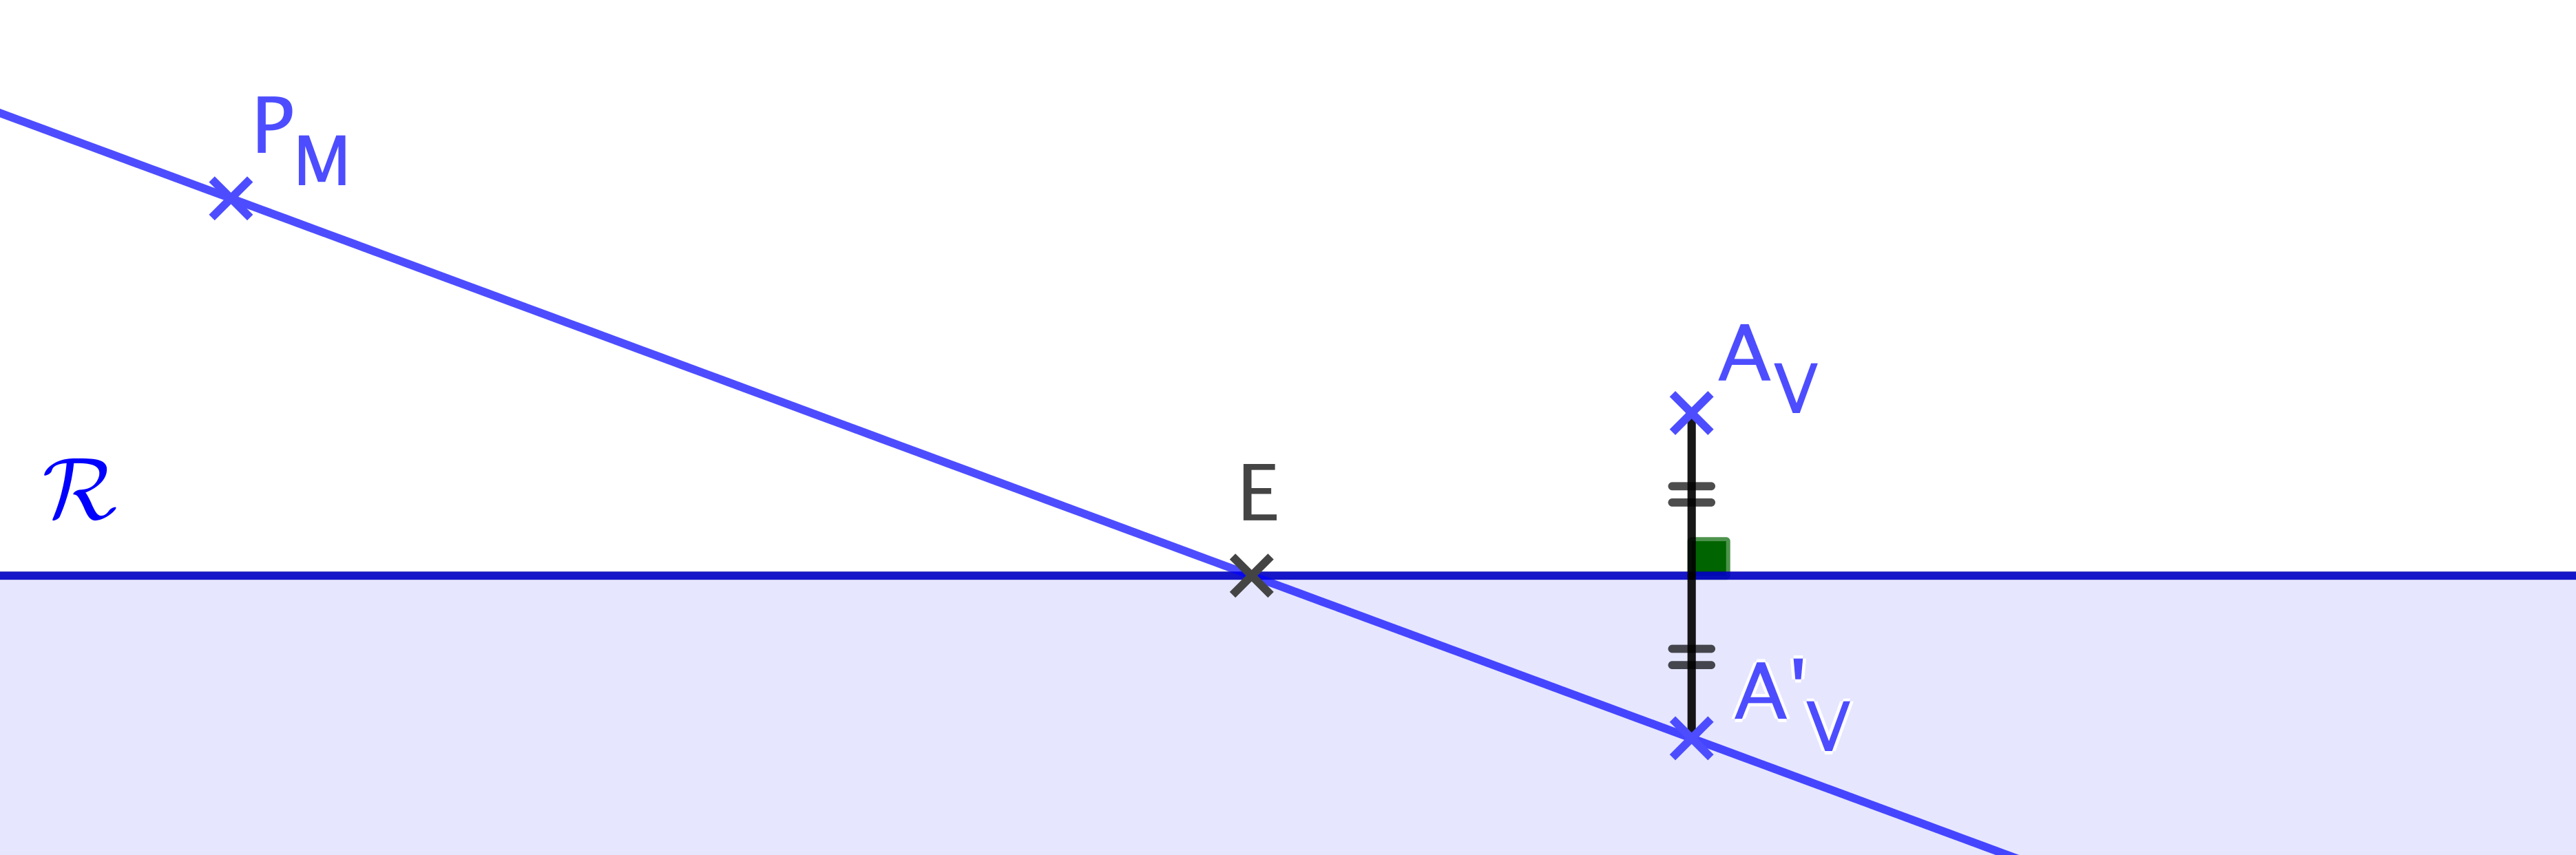
\includegraphics[scale = .6]{river-pb-geo-sol.png}}
\end{center}


\medskip


L'idée géniale consiste à tracer $A_V^\prime$ le symétrique orthogonal de $A_V$ par rapport à $\setproba{R}$ . Comme les longueurs sont conservées par symétrie orthogonale, quelque soit la forme du chemin le plus court entre $P_M$ et $A_V$ qui coupe au moins une fois $\setproba{R}$ , en restant toujours du même côté de la rive, on peut lui associer un chemin le plus court allant de $P_M$ à $A_V^\prime$ , cette association étant réciproque. Il ne reste plus à se souvenir que le chemin le plus court entre deux points du plan, sans contrainte, est une droite.


\medskip


Bien que très jolie, la solution ci-dessus ne tient pas compte de l'effort à fournir pour amener le seau d'eau depuis la rivière jusqu'à l'abreuvoir. De plus, que faire si l'on doit utiliser plusieurs fois le seau ? Avec cette contrainte de portage en tête, la solution est immédiate. La voici représentée.

\smallskip
\begin{center}
	\fbox{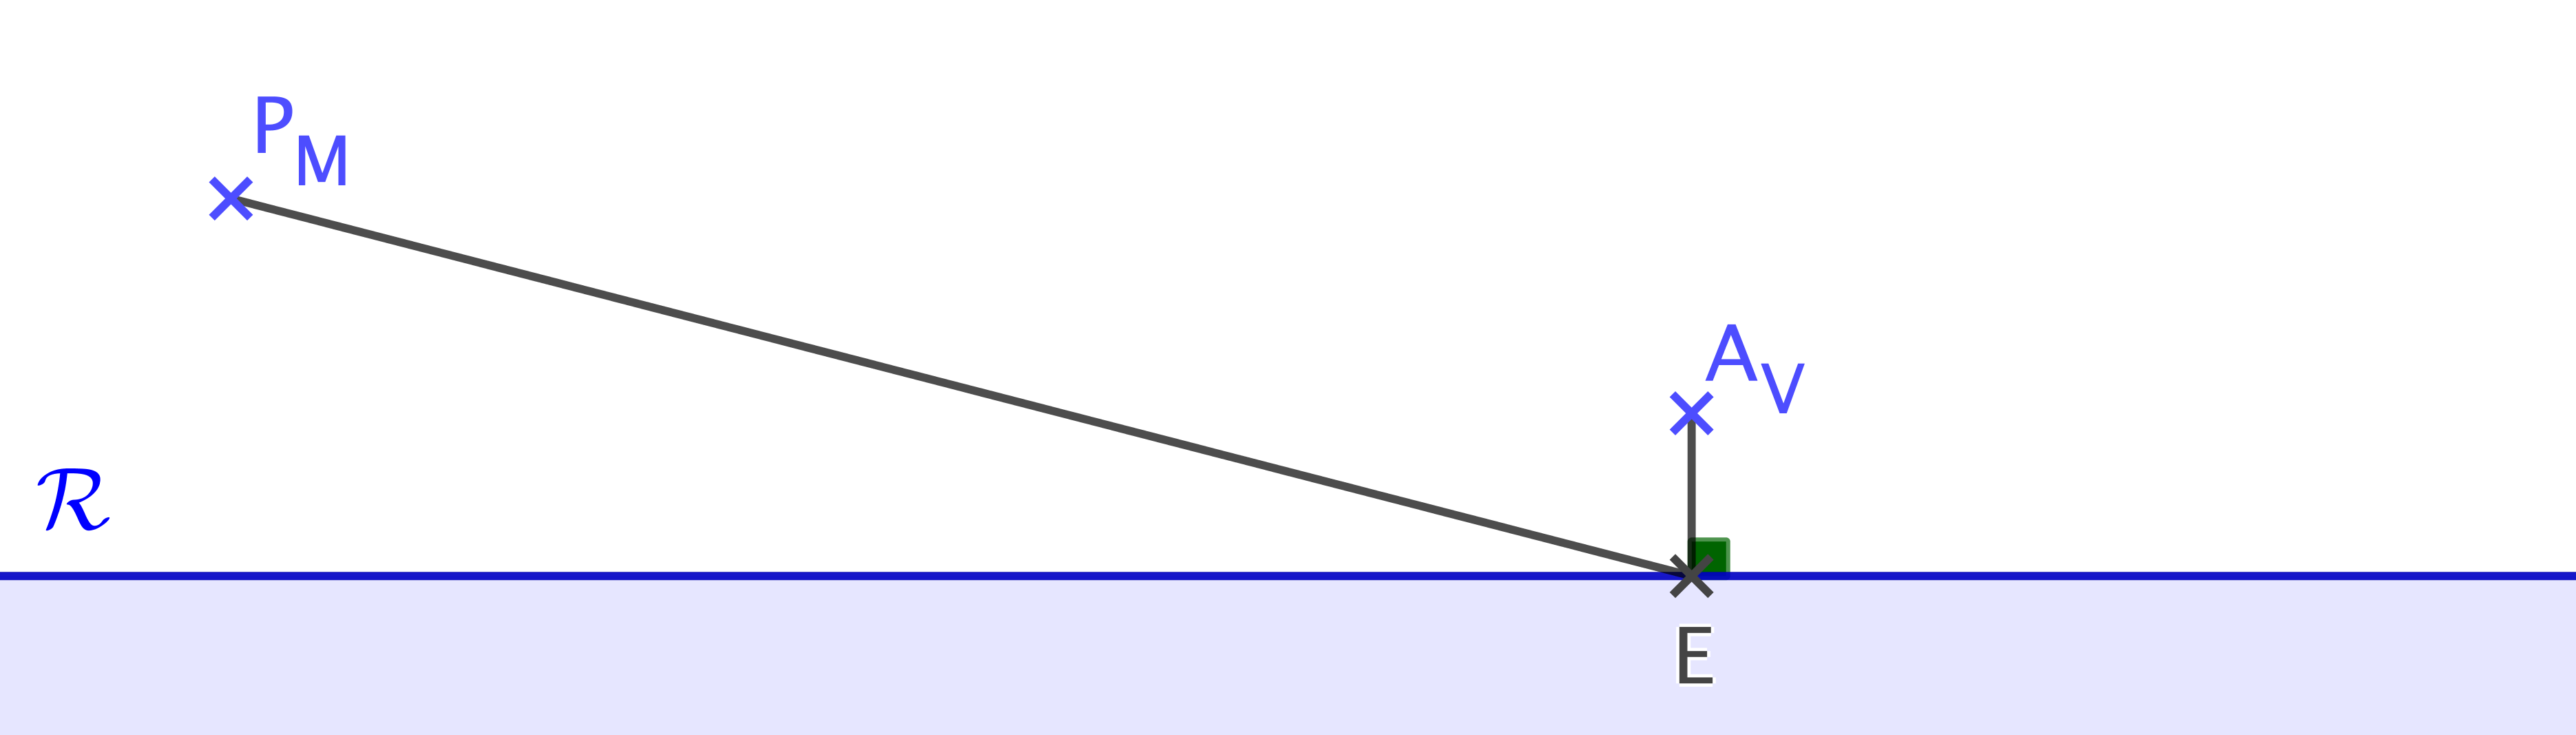
\includegraphics[scale = .6]{river-pb-practical-sol.png}}
\end{center}